\chapter{Progettazione logica} \label{chap:progettazione_logica}
	
	La progettazione logica permette di determinare lo schema logico del DW. Mentre durante la fase di progettazione concettuale viene ritagliata la porzione del dominio applicativo che dovrà essere considerato, con la fase di progettazione logica si determinano le strutture dati che andranno a rappresentare il DW stesso.\\
	In questo scenario, l'obiettivo primario è quindi di massimizzare la velocità di reperimento dei dati.\\
	
	\section{Schema di fatto} \label{sec:schema_fatto}
		La prima fase della progettazione logica consiste nel dare luogo allo schema che rappresenta l'albero degli attributi. Nello schema seguente (Figura \ref{fig:factschema}) la parte centrale esprime il ``fatto'' (\textit{fact}, in inglese), ovvero ciò a cui è volta la costruzione del modello. I campi del \textit{fatto} rappresentano le misure a cui si fa riferimento per correlare le dimensioni dello schema, che sono ottenute dalla disaggregazione iniziale dei \textit{dataset}.
		
		
		\begin{figure}[h!]
			\centering
				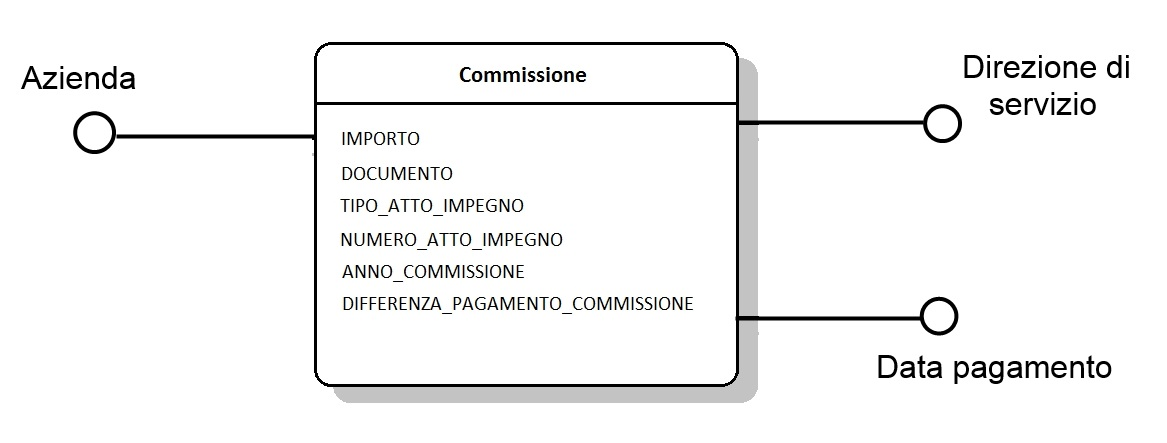
\includegraphics[scale=0.4]{factschema.jpg}
			\caption{Fact-Schema.}
			\label{fig:factschema}
		\end{figure}
		
		
		Uno schema di fatto può essere modellato in ambito relazionale mediante uno schema a stella in cui la cosiddetta \textit{fact table} (\textit{tabella di fatto}) contiene tutte le misure e gli attributi descrittivi direttamente collegati al fatto e nella quale, per ogni gerarchia presente, viene creata una \textit{dimension table} (\textit{tabella dimensionale}) che ne contiene tutti gli attributi.
	
	\section{Schema a stella} \label{sec:schema_stella}
	
		Lo schema a stella rappresenta il rapporto tra le dimensioni del modello e la \textit{fact table} (posta al centro della stella), che andrà a contenere le chiavi inter-dimensionali (indicate nella Figura \ref{fig:starschema} con un simbolo) le quali costituiscono i punti di contatto tra le dimensioni considerate.
		Questo schema a stella permette efficacemente di rappresentare un cubo dimensionale, incentrato sul fatto di interesse del processo decisionale o di analisi. Lo schema ed il cubo rappresentano quindi un insieme di eventi, descritti quantitativamente da misure numeriche. Ogni asse del cubo (ogni dimensione) rappresenta una possibile dimensione di analisi e ciascuna dimensione può essere vista a più livelli di dettaglio, individuati dagli attributi strutturati in gerarchie.
		
		\begin{figure}[h!]
			\centering
				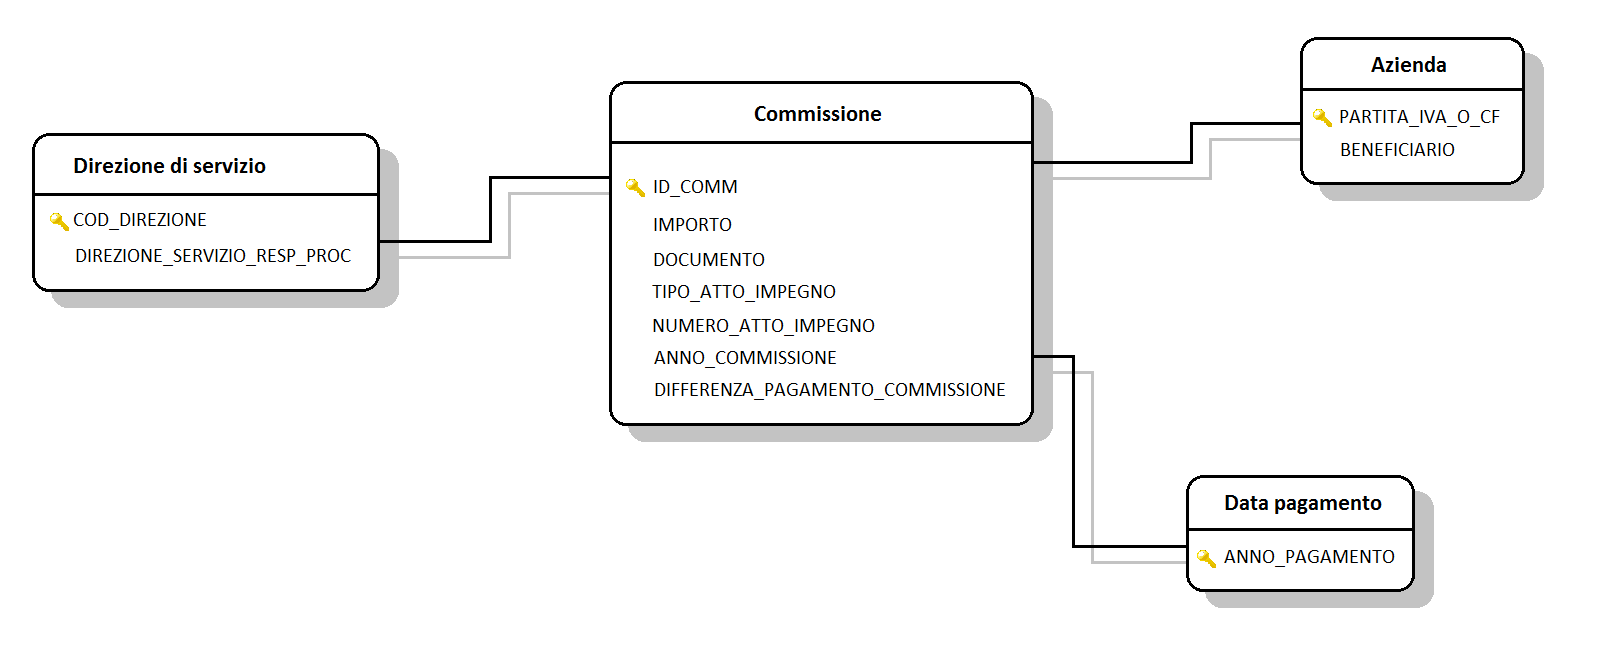
\includegraphics[scale=0.45]{starschema.jpg}
			\caption{Star-Schema.}
			\label{fig:starschema}
		\end{figure}
		
	
	\section{Flat Table} \label{sec:flat_table}
	
		Fin'ora abbiamo parlato di modelli logici a supporto dei nostri dati, come schemi relazionali, concettuali e a stella. Facendo un passo avanti, entriamo quindi nell'ambito dell'implementazione effettiva di questi schemi logici, introducendo il concetto di \textit{Flat Table}: una \textit{Flat Table}, o \textit{Flat-File Database} è un unico file di testo, contenente soltanto dati e delimitatori, che, privo di qualsiasi tipo di riferimento relazionale, rappresenta in concreto il nostro database.\\
		\\
		Nel nostro caso, il file \texttt{.csv} ottenuto come risultato del processo di \textit{Data Integration} sarà allora il supporto ``fisico'' per il nostro database. Questo file, denominato \texttt{Commissioni.csv}, sarà di fatto un unico, enorme file contenente sia i dati della \textit{fact table} sia i dati di tutte le \textit{dimension table} presenti nello schema di fatto. In questo modo viene eliminata ogni tipo di relazione (o se vogliamo, collegamento) tra i dati da analizzare, rendendo necessario più spazio per la memorizzazione ma migliorando notevolmente le tempistiche in fase di analisi.\\
		In Figura \ref{fig:flat_table} possiamo vedere le prime righe e colonne del file \texttt{Commissioni.csv} sopra citato. Per le trasformazioni di \textit{Data Integration} che generano tale file si veda il Capitolo \ref{chap:elaborazione}.
		
		\begin{figure}[h!]
			\centering
				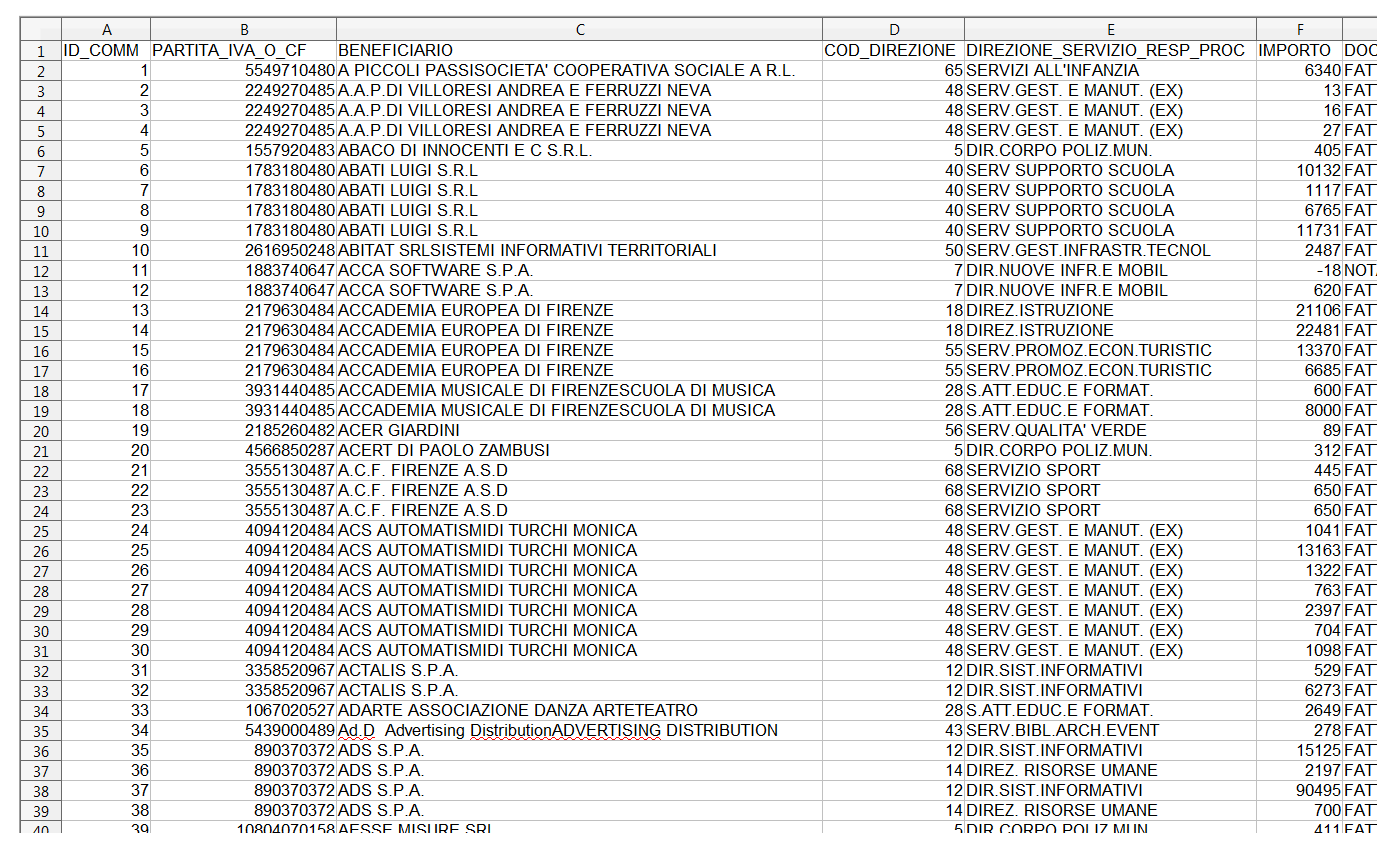
\includegraphics[scale=0.5]{flat_table.png}
			\caption{\textit{Flat Table} finale.}
			\label{fig:flat_table}
		\end{figure}
